\documentclass{article}

\usepackage[margin=1in]{geometry}
\usepackage{wrapfig}
\usepackage{tkz-euclide}
\usepackage{siunitx}
\usepackage{amsmath}

\title{2021 Castro Valley Junior Math Tournament Solutions}
\author{}
\date{}

\begin{document}
\maketitle

\section*{Mooving Cow}
\begin{wrapfigure}{r}{0.35\linewidth}
	\centering
	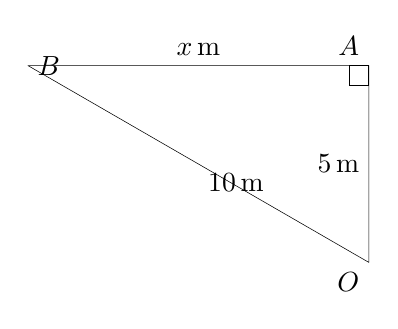
\begin{tikzpicture}
		\tkzDefPoints{0/0/O,0/2.5/A}
		\tkzDefShiftPoint[A](1,0){b}

		\tkzInterLC[R](A,b)(O,5cm)
		\tkzGetSecondPoint{B}

		\tkzDrawPolygon(O,A,B)
		\tkzLabelPoints[below left](O)
		\tkzLabelPoints[above left](A)
		\tkzLabelPoints[right](B)
		\tkzLabelLine[left](O,A){$\SI{5}{m}$}
		\tkzLabelLine[below right](O,B){$\SI{10}{m}$}
		\tkzLabelLine[above](A,B){$\SI[parse-numbers=false]{x}{m}$}
		\tkzMarkRightAngle(O,A,B)
	\end{tikzpicture}
\end{wrapfigure}
If we plot the position of FJ's house ($O$), Bessie's starting position ($A$), and Bessie's position when she is exactly $10$ meters away from the house ($B$), we can see that the points form a right triangle.
We can use the Pythagorean theorem to find $x$, which is how far Bessie moved in meters.
$x^2 + 5^2 = 10^2$, so $x^2 = 100 - 25 = 75$ and $x = \sqrt{75}$.
Time is distance divided by speed and Bessie moved at $2$ meters per second, so it took her $\frac{\sqrt{75}}{2}$ seconds to get $10$ meters away from the house.
The square root can be simplified since $75$ is a multiple of a perfect square, so the final answer is
\[
	\frac{\sqrt{75}}{2} = \frac{\sqrt{25 \cdot 3}}{2} = \frac{\sqrt{25}\sqrt{3}}{2} = \boxed{\frac{5\sqrt{3}}{2}}
\]
Alternatively, we can also use the special right triangle ratios instead of the Pythagorean theorem.
This right triangle is a $30$-$60$-$90$ triangle because $OA$ is half of $OB$.
In a $30$-$60$-$90$ triangle, the length of the longer leg is $\sqrt{3}$ times the length of the shorter leg, so $x = 5\sqrt{3}$ and we also get $\frac{5\sqrt{3}}{2}$ seconds as the answer.

\section*{Cowangle}
There are several ways to solve this problem.
The most direct way is to use the inverse Pythagorean theorem, which states that in a right triangle like this where we drew an altitude from the right angle to the hypotenuse, $\frac{1}{AB^2} + \frac{1}{AC^2} = \frac{1}{AX^2}$.
$\frac{1}{7^2} + \frac{1}{10^2} = \frac{1}{AX^2}$, so $\frac{1}{AX^2} = \frac{1}{49} + \frac{1}{100} = \frac{149}{4900}$ and $AX = \sqrt{\frac{1}{\frac{149}{4900}}} = \sqrt{\frac{4900}{149}} = \frac{70}{\sqrt{149}}$.
To fully simplify this, we need to rationalize the denominator by multiplying both the top and the bottom by $\sqrt{149}$.
On the top we have $70\sqrt{149}$ and on the bottom we have $\sqrt{149}\sqrt{149} = \sqrt{149}^2 = 149$, so the answer is \fbox{$\frac{70\sqrt{149}}{149}$}.

\section*{Mooish}
Annabelle and Cornelius were both asked about Betsie's type and they gave different answers, so one of them must be telling the truth and the other must be lying.
This means that their types are different, therefore Betsie is lying, meaning that she is falsy.
Annabelle told the truth about Betsie's type, so she is truthy, and Cornelius lied about Betsie's type, so she is falsy.

\section*{Green Cows}
First, we find the grass chowing rates of Bessie and Elsie.
Bessie can chow all the grass in a field in $3 \cdot 60 = 180$ minutes, so she can chow $\frac{1}{180}$ fields per minute.
Similarly, Elsie can chow $\frac{1}{4}$ fields per minute.
Together, they can chow $\frac{1}{180} + \frac{1}{4} = \frac{23}{90}$ fields per minute, so it takes them \fbox{$\frac{90}{23}$ minutes or $\frac{3}{46}$ hours} to chow one field.
\end{document}
